\documentclass[14pt]{extbook}
\usepackage{multicol, enumerate, enumitem, hyperref, color, soul, setspace, parskip, fancyhdr} %General Packages
\usepackage{amssymb, amsthm, amsmath, bbm, latexsym, units, mathtools} %Math Packages
\everymath{\displaystyle} %All math in Display Style
% Packages with additional options
\usepackage[headsep=0.5cm,headheight=12pt, left=1 in,right= 1 in,top= 1 in,bottom= 1 in]{geometry}
\usepackage[usenames,dvipsnames]{xcolor}
\usepackage{dashrule}  % Package to use the command below to create lines between items
\newcommand{\litem}[1]{\item#1\hspace*{-1cm}\rule{\textwidth}{0.4pt}}
\pagestyle{fancy}
\lhead{Progress Quiz 10}
\chead{}
\rhead{Version A}
\lfoot{6232-9639}
\cfoot{}
\rfoot{Fall 2020}
\begin{document}

\begin{enumerate}
\litem{
Write the equation of the graph presented below in the form $f(x)=ax^2+bx+c$, assuming  $a=1$ or $a=-1$. Then, choose the intervals that $a, b,$ and $c$ belong to.
\begin{center}
    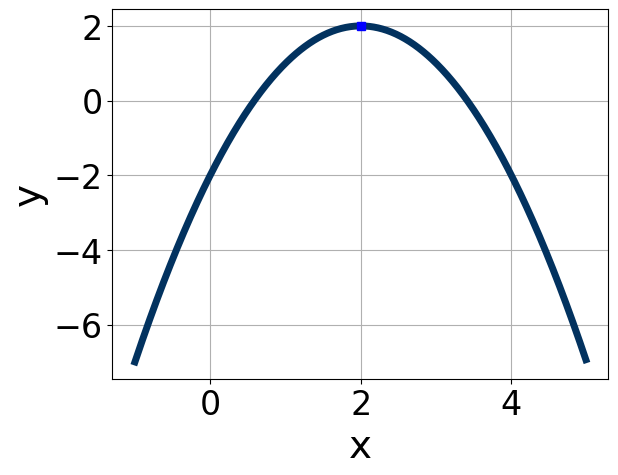
\includegraphics[width=0.5\textwidth]{../Figures/quadraticGraphToEquationA.png}
\end{center}
\begin{enumerate}[label=\Alph*.]
\item \( a \in [-2.6, 0.2], \hspace*{5mm} b \in [4, 5], \text{ and } \hspace*{5mm} c \in [-5, 1] \)
\item \( a \in [-2.6, 0.2], \hspace*{5mm} b \in [-4, -2], \text{ and } \hspace*{5mm} c \in [-5, 1] \)
\item \( a \in [-0.8, 2.4], \hspace*{5mm} b \in [-4, -2], \text{ and } \hspace*{5mm} c \in [5, 7] \)
\item \( a \in [-0.8, 2.4], \hspace*{5mm} b \in [4, 5], \text{ and } \hspace*{5mm} c \in [5, 7] \)
\item \( a \in [-2.6, 0.2], \hspace*{5mm} b \in [-4, -2], \text{ and } \hspace*{5mm} c \in [-8, -5] \)

\end{enumerate} }
\litem{
Graph the equation below.\[ f(x) = (x+2)^2 - 17 \]\begin{enumerate}[label=\Alph*.]
\begin{multicols}{2}\item 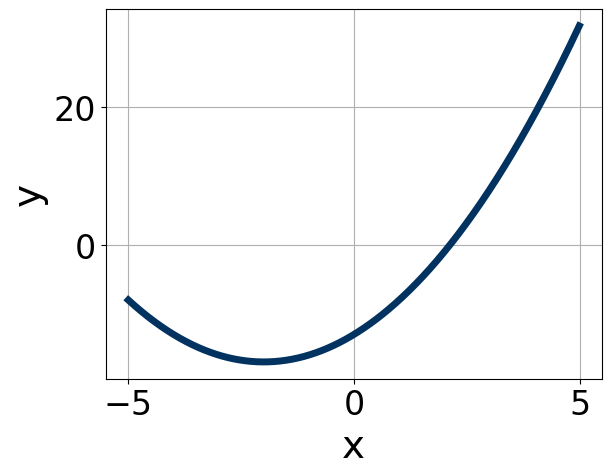
\includegraphics[width = 0.3\textwidth]{../Figures/quadraticEquationToGraphCopyAA.png}\item 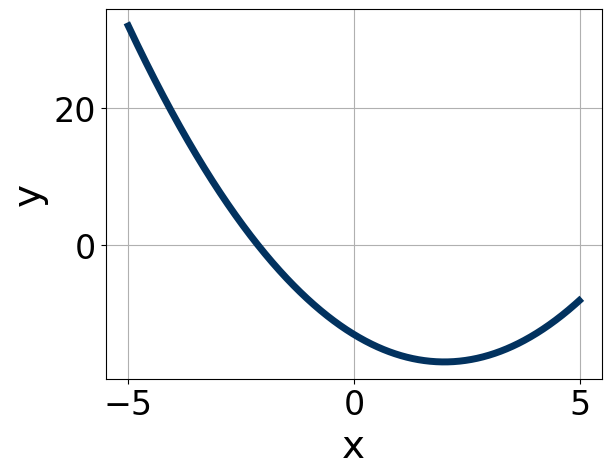
\includegraphics[width = 0.3\textwidth]{../Figures/quadraticEquationToGraphCopyBA.png}\item 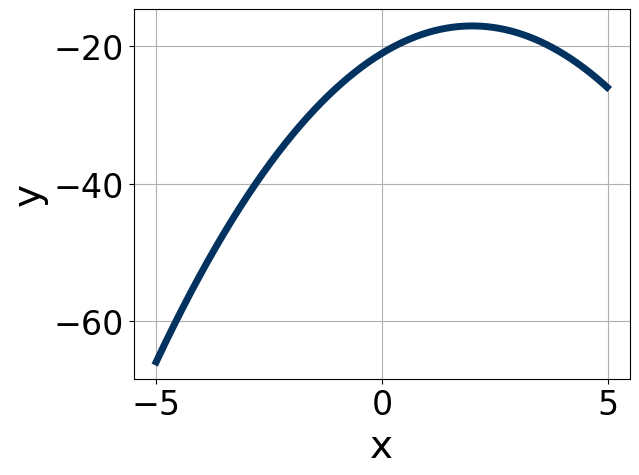
\includegraphics[width = 0.3\textwidth]{../Figures/quadraticEquationToGraphCopyCA.png}\item 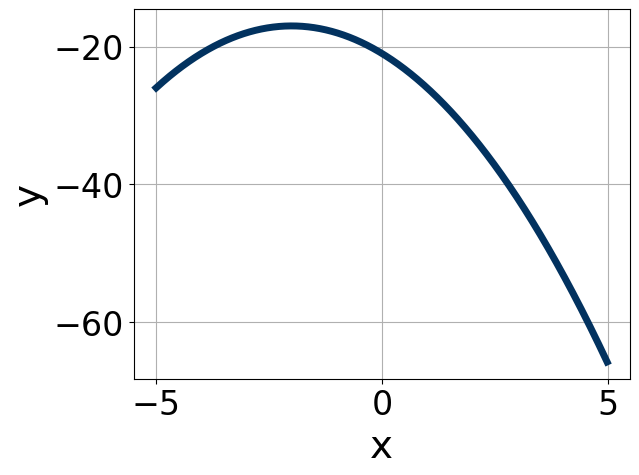
\includegraphics[width = 0.3\textwidth]{../Figures/quadraticEquationToGraphCopyDA.png}\end{multicols}\item None of the above.
\end{enumerate} }
\litem{
Graph the equation below.\[ f(x) = (x+3)^2 - 15 \]\begin{enumerate}[label=\Alph*.]
\begin{multicols}{2}\item 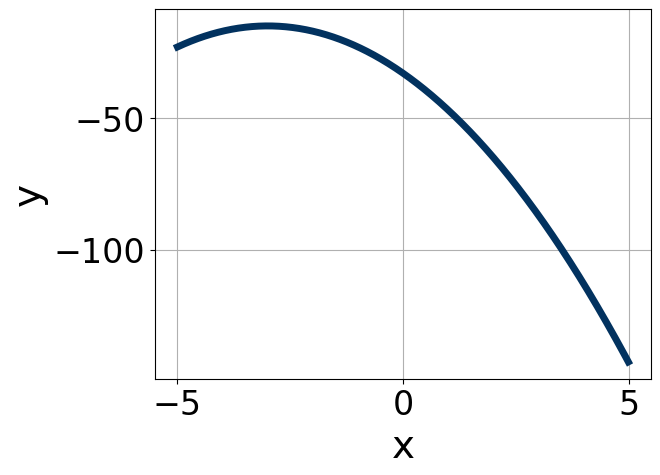
\includegraphics[width = 0.3\textwidth]{../Figures/quadraticEquationToGraphAA.png}\item 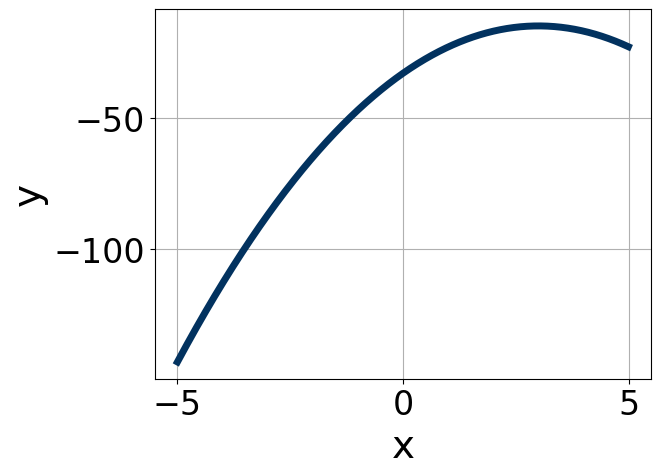
\includegraphics[width = 0.3\textwidth]{../Figures/quadraticEquationToGraphBA.png}\item 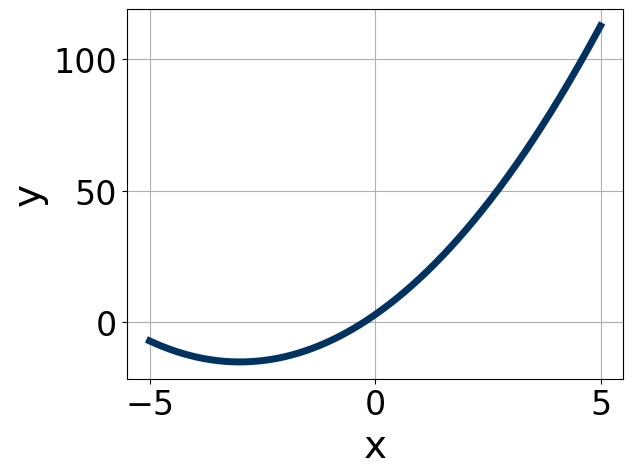
\includegraphics[width = 0.3\textwidth]{../Figures/quadraticEquationToGraphCA.png}\item 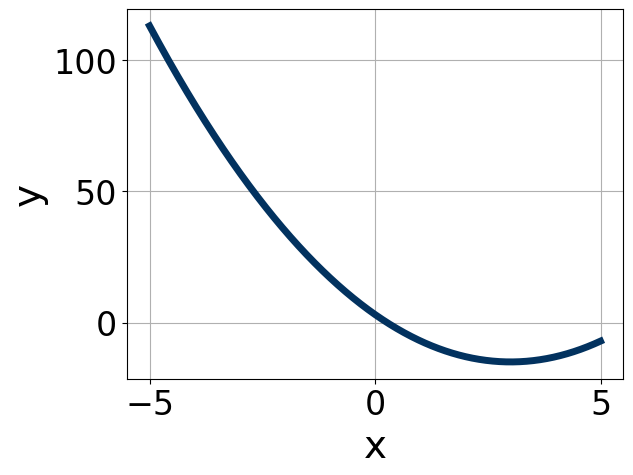
\includegraphics[width = 0.3\textwidth]{../Figures/quadraticEquationToGraphDA.png}\end{multicols}\item None of the above.
\end{enumerate} }
\litem{
Factor the quadratic below. Then, choose the intervals that contain the constants in the form $(ax+b)(cx+d); b \leq d.$\[ 36x^{2} -7 x -15 \]\begin{enumerate}[label=\Alph*.]
\item \( a \in [3, 5.5], \hspace*{5mm} b \in [-5, -1], \hspace*{5mm} c \in [8.5, 9.5], \text{ and } \hspace*{5mm} d \in [4, 8] \)
\item \( a \in [9.6, 14.2], \hspace*{5mm} b \in [-5, -1], \hspace*{5mm} c \in [2.6, 3.2], \text{ and } \hspace*{5mm} d \in [4, 8] \)
\item \( a \in [1.9, 2.2], \hspace*{5mm} b \in [-5, -1], \hspace*{5mm} c \in [17.5, 21.4], \text{ and } \hspace*{5mm} d \in [4, 8] \)
\item \( a \in [0, 1.6], \hspace*{5mm} b \in [-29, -24], \hspace*{5mm} c \in [0.9, 1.2], \text{ and } \hspace*{5mm} d \in [18, 22] \)
\item \( \text{None of the above.} \)

\end{enumerate} }
\litem{
Factor the quadratic below. Then, choose the intervals that contain the constants in the form $(ax+b)(cx+d); b \leq d.$\[ 36x^{2} +47 x + 15 \]\begin{enumerate}[label=\Alph*.]
\item \( a \in [0.59, 1.39], \hspace*{5mm} b \in [18, 26], \hspace*{5mm} c \in [0.5, 1.2], \text{ and } \hspace*{5mm} d \in [27, 31] \)
\item \( a \in [11.63, 12.83], \hspace*{5mm} b \in [2, 7], \hspace*{5mm} c \in [1.9, 3.3], \text{ and } \hspace*{5mm} d \in [4, 10] \)
\item \( a \in [1.43, 3.38], \hspace*{5mm} b \in [2, 7], \hspace*{5mm} c \in [17.8, 19.2], \text{ and } \hspace*{5mm} d \in [4, 10] \)
\item \( a \in [3.54, 4.16], \hspace*{5mm} b \in [2, 7], \hspace*{5mm} c \in [8, 10.3], \text{ and } \hspace*{5mm} d \in [4, 10] \)
\item \( \text{None of the above.} \)

\end{enumerate} }
\litem{
Write the equation of the graph presented below in the form $f(x)=ax^2+bx+c$, assuming  $a=1$ or $a=-1$. Then, choose the intervals that $a, b,$ and $c$ belong to.
\begin{center}
    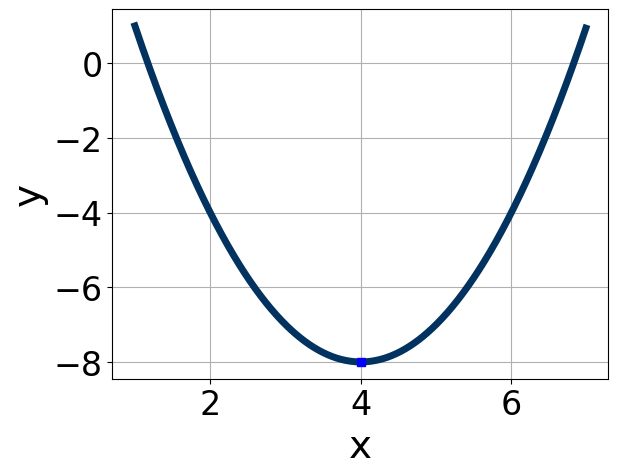
\includegraphics[width=0.5\textwidth]{../Figures/quadraticGraphToEquationCopyA.png}
\end{center}
\begin{enumerate}[label=\Alph*.]
\item \( a \in [0, 3], \hspace*{5mm} b \in [4, 11], \text{ and } \hspace*{5mm} c \in [24, 25] \)
\item \( a \in [0, 3], \hspace*{5mm} b \in [4, 11], \text{ and } \hspace*{5mm} c \in [4, 9] \)
\item \( a \in [-1, 0], \hspace*{5mm} b \in [4, 11], \text{ and } \hspace*{5mm} c \in [-25, -22] \)
\item \( a \in [0, 3], \hspace*{5mm} b \in [-8, -7], \text{ and } \hspace*{5mm} c \in [4, 9] \)
\item \( a \in [-1, 0], \hspace*{5mm} b \in [-8, -7], \text{ and } \hspace*{5mm} c \in [-25, -22] \)

\end{enumerate} }
\litem{
Solve the quadratic equation below. Then, choose the intervals that the solutions belong to, with $x_1 \leq x_2$ (if they exist).\[ -20x^{2} +7 x + 8 = 0 \]\begin{enumerate}[label=\Alph*.]
\item \( x_1 \in [-0.56, -0.1] \text{ and } x_2 \in [0.8, 0.86] \)
\item \( x_1 \in [-16.86, -16.46] \text{ and } x_2 \in [9.38, 9.96] \)
\item \( x_1 \in [-1.38, -0.63] \text{ and } x_2 \in [0.41, 0.61] \)
\item \( x_1 \in [-26.19, -25.79] \text{ and } x_2 \in [26.14, 26.68] \)
\item \( \text{There are no Real solutions.} \)

\end{enumerate} }
\litem{
Solve the quadratic equation below. Then, choose the intervals that the solutions $x_1$ and $x_2$ belong to, with $x_1 \leq x_2$.\[ 20x^{2} -69 x + 54 = 0 \]\begin{enumerate}[label=\Alph*.]
\item \( x_1 \in [0.68, 0.9] \text{ and } x_2 \in [2.73, 3.76] \)
\item \( x_1 \in [23.95, 24.04] \text{ and } x_2 \in [44.61, 45.16] \)
\item \( x_1 \in [0.37, 0.44] \text{ and } x_2 \in [6.25, 6.81] \)
\item \( x_1 \in [1.17, 1.22] \text{ and } x_2 \in [2.19, 2.29] \)
\item \( x_1 \in [0.42, 0.57] \text{ and } x_2 \in [5.82, 6.18] \)

\end{enumerate} }
\litem{
Solve the quadratic equation below. Then, choose the intervals that the solutions $x_1$ and $x_2$ belong to, with $x_1 \leq x_2$.\[ 10x^{2} -57 x + 54 = 0 \]\begin{enumerate}[label=\Alph*.]
\item \( x_1 \in [0.73, 0.97] \text{ and } x_2 \in [5.31, 7.23] \)
\item \( x_1 \in [1, 1.48] \text{ and } x_2 \in [4.04, 4.62] \)
\item \( x_1 \in [11.68, 12.21] \text{ and } x_2 \in [44.23, 46.73] \)
\item \( x_1 \in [0.06, 0.66] \text{ and } x_2 \in [13.37, 13.76] \)
\item \( x_1 \in [2.21, 2.42] \text{ and } x_2 \in [1.93, 3.85] \)

\end{enumerate} }
\litem{
Solve the quadratic equation below. Then, choose the intervals that the solutions belong to, with $x_1 \leq x_2$ (if they exist).\[ 19x^{2} -9 x -8 = 0 \]\begin{enumerate}[label=\Alph*.]
\item \( x_1 \in [-9.54, -8.49] \text{ and } x_2 \in [17.31, 18.22] \)
\item \( x_1 \in [-1.18, -0.48] \text{ and } x_2 \in [0.27, 0.68] \)
\item \( x_1 \in [-26.08, -25.91] \text{ and } x_2 \in [25.83, 27.62] \)
\item \( x_1 \in [-0.51, -0.07] \text{ and } x_2 \in [0.78, 1.65] \)
\item \( \text{There are no Real solutions.} \)

\end{enumerate} }
\end{enumerate}

\end{document}